\section{Background}
\label{sec:background}

\subsection{The Problem}
\label{subsec:the_problem}

Throughout Sqlite's history many tests, papers, and tools have been developed in order to understand, and modify the future direction of Sqlite. However, when a user wants to understand at a deeper level how Sqlite is working or finding obscure bugs, they are stuck with manually trawling through a Hex editor. This paper aims to solve this by providing a visualisation of the internal structure, as well as a update log that is updated in real time, when the database is modified.


\subsection{Sqlite}
\label{subsec:sqlite}

\subsubsection{What is Sqlite}
\label{subsubsec:what_is_sqlite}

Sqlite is a single self-contained, serverless SQL database engine. Started on 29 May 2000 by D. Richard Hipp \citep{sqlite} from gathered inspiration while working on software for guided missiles on a battleship where they needed a self-contained portable database. \citep{sqlitedefguide} He joined up with Joe Mistachkin followed by Dan Kennedy in 2002. Version 1.0 was released in August 2000, then in just over year on the 28 November 2001 2.0 which introduced, BTrees and many of the features seen in 3.0. Which came a lot later containing a full rewrite and improvement over 2.0, with the first public release on 18 June 2004. At the time of writing this paper we are currently sitting at version 3.10.4 \citep{sqlite}.
\\\\
Sqlite is open source within the public domain making it accessible to everyone. The entire library size can be 350Kib, with some option features omitted it could be reduced to around 300Kib making it incredibly small compared to what it does. In addition to this the runtime usage is minimal with 4Kib stack space and 100Kib heap, allowing it to run on almost anything. Sqlite's main strength is that the entire database in encoded into a single portable file, that can be read, on any system whether 32 or 64 bit, big or small endian. It is often seen as a replacement for storage files rather then a database system \citep{sqlite}.

\subsubsection{Where is Sqlite used}
\label{subsubsec:where_is_sqlite}

As Sqlite is a minimal portable database engine it has primarily two uses, The first as a relation database like any other, the second as a application file format. In the former case Sqlite would be set up the same way a tradition database system would be, with the primary purpose to hold the back end storage information. The latter case is more unique to Sqlite and is what sets it apart from the traditional database engines \citep{sqlite}. Because of this Sqlite is used everywhere, a few of the big names include, apple, android, adobe even a special version was produced specifically for windows 10. In fact Sqlite might be the single most deployed software currently \citep{sqlite, sqlitetalk}.

\subsubsection{How is Sqlite works}
\label{subsubsec:how_sqlite_works}

Sqlite consist of three main parts, the backend, core and the SQL compiler. Figure~\ref{fig:sqlite_arch} shows the architectural digram of Sqlite.

\begin{figure}[H]
	\centering
	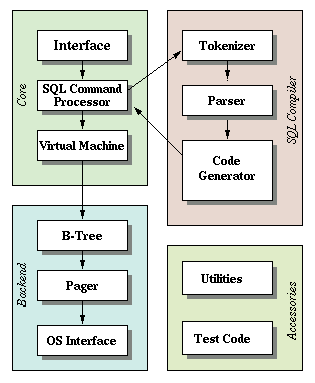
\includegraphics[scale=0.5]{images/sqlite_arch.png}
	\caption{Sqlite architectural diagram \citep{sqlite}}
	\label{fig:sqlite_arch}
\end{figure}

The SQL compiler is designed to take SQL strings and turn them into valid SQL commands, it is made up of three parts. Firstly the tokenizer takes a string containing SQL statements and turns it into tokens passing them one by one to the parser. The parser takes the tokens and assign meaning to them. Lastly the code generator takes the tokens from the parser and assembles complete SQL statements that are to be ran on the database file.
\\\\
The Core itself is actually a virtual machine implementing a specifically designed computing engine to manipulate database files. The interface module defines the interface between the virtual machine and the SQL library including the external API. Knowing this we can see that the virtual machine takes the code output from the code generator to manipulate the backend / database. 
\\\\
The final main module is the backend which is the main focus of this paper, controlling the file format. The OS interface contains an abstraction layer to write the files to disk or memory. The Pager takes the B-Trees and is responsible for reading, writing and caching them. This involves locking, rollback and atomic commits of the database. Sqlite uses a B-Tree system to navigate and store the data on disk, this module contains the implementation of the B-tree and as such the defines the file format. 
\\\\
The last module, accessories is made up of two parts. Utility containing functions that are used all around Sqlite, such as memory allocation, string comparison, random number generator and symbol tables. The test section contains all the test scripts and only exist for testing purposes, of which contains over 811 times more code then the actual project.

\subsection{The Sqlite file format}
\label{subsec:sqlite_file_format}

\subsubsection{The page system}
\label{subsubsec:sqlite_page_system}

As mentioned is section~\ref{subsubsec:how_sqlite_works} Sqlite works off of a B-tree structure to store and navigate the database. The B-Tree implementation is designed to support fast querying, the various B-Tree structures can be found in \cite{btreepaper} paper. Sqlite also takes some improvements seen in \cite{btreeimprpaper} book \citep{sqliteray}.
\\\\
The basic idea is that the file is made up of chunks or pages, each page is the same fixed size. The size of the pages are a power of two between 512 - 65536 bytes. Pages are numbered starting with 1 instead of 0. The maximum number of pages that Sqlite can hold is 2,147,483,646 with a page size of 512 bytes witch is around 140 terabytes. The minimum number of pages within a database is 1. There are five types of pages:

\begin{itemize} 
	\item Lock Byte Page \hfill \\
		The lock byte page appears between bytes, 1073741824 - 1073742335, if a database is smaller or equal to 1073742335 bytes it will not contain a lock byte page. It is used by the OS Interface mentioned in section~\ref{subsubsec:how_sqlite_works}.
	
	\item Freelist Page \hfill \\
		The freelist page is a unused page, often left behind when information is deleted from the database. The other type is a freelist trunk page containing page numbers of the other freelist pages.
	
	\item B-Tree Page \hfill \\
		The B-Tree page, contains one of the four types of B-Trees, more in section~\ref{subsubsec:sqlite_trees_and_cells}.
	
	\item Payload overflow page \hfill \\
		The payload overflow page is created to hold the remaining payload from a B-Tree cell when the payload is to large.
	
	\item Pointer map page \hfill \\
		Pointer map pages are inserted to make the vacuum modes faster. And are the reverse B-Tree going child to parent rather then parent to child. They exist in databases that have a non-zero value largest root B-Tree within the header. The first instance of these pages are at page 2. 
\end{itemize} 

\subsubsection{The Header}
\label{subsubsec:sqlite_page_hader}

The first page before the root B-Tree contains a 100 byte header. This is what makes Sqlite have zero configuration as all the database settings are stored within this header, all multibyte fields are stored in a big-endian format. The header follows the following format: 

\begin{longtable}[h]{| c | c | p{10cm} |}
		\hline
			\textbf{Byte Offset} & \textbf{Byte Size} & \textbf{Description} \\ 
		\hline
		\endhead
			0 & 16 & A UTF-8 Header String followed by null terminator read as: "SQLite format 3" or in hex: "53 51 4c 69 74 65 20 66 6f 72 6d 61 74 20 33 00". \\
		\hline
			16 & 2 & Page Size 	in bytes, power of two between 512 - 65536 bytes. if using version 3.7.0.1 and earlier between 512 - 32768, or 1 for 65536. \\
		\hline
			18 & 1 & Write version, 1 for legacy; 2 for WAL. \\
		\hline
			19 & 1 & Read version, 1 for legacy; 2 for WAL. \\
		\hline
			20 & 1 & Bytes of unused space at the end of each page. This space is used by extensions, such as cryptographic to store a checksum, but normally 0. \\
		\hline
			21 & 1 & Maximum embedded payload fraction, must be 64. Was going to be used to determine the maximum size of a B-Tree cell on a index B-Tree. \\
		\hline
			22 & 1 & Minimum embedded payload fraction, must be 32. Was going to be used to determine the portion of a B-Tree cell that has one or more overflow pages on a index B-tree. \\
		\hline
			23 & 1 & Leaf payload fraction, must be 32. Was going to be used to determine the portion of a B-Tree cell that has one or more overflow pages on a leaf or table B-Tree. \\
		\hline
			24 & 4 & File change counter. It counts the number of times the database is unlocked after being modified. May not be incremented in WAL mode. \\
		\hline
			28 & 4 & Size of the database in pages, Total number of pages. \\
		\hline
			32 & 4 & Page number of first freelist page, or 0 if no freelist. \\
		\hline
			36 & 4 & Number of freelist pages. \\
		\hline
			40 & 4 & Schema Cookie. The schema version, each time the schema is modified this number is incremented. \\
		\hline
			44 & 4 & Schema format number. either 1, 2, 3 or 4. \newline
			1. Format support back to version 3.0.0. \newline
			2. Varying number of columns within the same table. From Version 3.1.3. \newline 
			3. Extra column can be non-NULL values. From Version 3.1.4. \newline
			4. Respects DESC keyword and boolean type. From Version 3.3.0. \newline \\
		\hline
			48 & 4 & Page cache size. suggestion only towards Sqlite's pager. \\
		\hline
			52 & 4 & Page number of largest root B-Tree, when in vacuum mode else 0. \\
		\hline
			56 & 4 & Text encoding. \newline
			 1 for UTF-8. \newline 
			 2 for UTF-816le. \newline 
			 3 for UTF-816be. \\
		\hline
			60 & 4 & User version. Set by and read by the user, not used by Sqlite. \\
		\hline
			64 & 4 & Incremental-vacuum mode. Non 0 for true. 0 for false \\
		\hline
			68 & 4 & Application ID. Used to associate the database with a application. 0 is Sqlite3 Database \\
		\hline
			72 & 20 & Empty, Reserved for expansion. \\
		\hline
			92 & 4 & Version-valid-for-number. Value of the change counter when the Sqlite version number was stored. \\
		\hline
			96 & 4 & Version. Sqlite version. \\
		\hline
	\caption{Sqlite Header, modified from \cite{sqlite}}
	\label{tbl:sqlite_header}
\end{longtable}

Immediately following the header is the root B-Tree which we will cover the the next section.

\subsubsection{The Trees and Cells}
\label{subsubsec:sqlite_trees_and_cells}

As mentioned in section~\ref{subsubsec:sqlite_page_system} the file is split into pages and each page contains one of four types of B-Tree. Each B-Tree type is slightly different but follow the same pattern. At the start of each page there is the B-Tree / page header. Following the header is a array of pointers to their cells. The cell layouts are where the main difference in B-Tree types become more apparent, as they store the payload. Figure~\ref{fig:sqlite_file_format} shows the full layout of the SQlite file.

\begin{figure}[H]
	\centering
	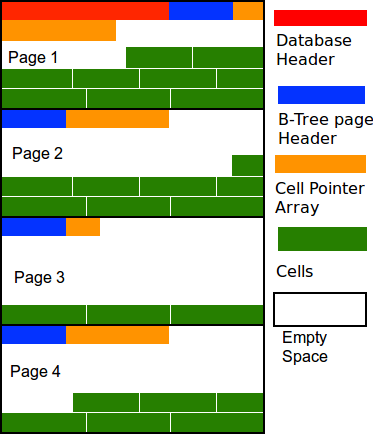
\includegraphics[scale=0.5]{images/sqlite_file_format.png}
	\caption{Sqlite file format, modified from \cite{sausagefactory}}
	\label{fig:sqlite_file_format}
\end{figure}

The cells start at the end of the page and work backwards towards the top.
\\\\
There are two main types of B-Trees. Table and Index, both of which uses a key-value system in order to organise them. The Table B-Trees use 64 bit integers also known as row-id or primary key. The Index B-Trees uses database records as keys. This can be seen in the following example taken from \cite{sqliteray}:

\begin{lstlisting}
 CREATE TABLE t1(a INTEGER PRIMARY KEY, b, c, d);
 CREATE INDEX i1 ON t1(d, c);

 INSERT INTO t1 VALUES(1, 'triangle', 3, 180, 'green');
 INSERT INTO t1 VALUES(2, 'square',   4, 360, 'gold');
 INSERT INTO t1 VALUES(3, 'pentagon', 5, 540, 'grey');
\end{lstlisting}

\begin{figure}[H]
	\centering
	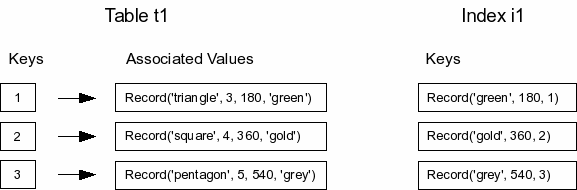
\includegraphics[scale=0.5]{images/examplepop.png}
	\caption{Example key pair database \citep{sqliteray}}
	\label{fig:sqlite_key_pair}
\end{figure}

Those two types of B-Trees are broken down into Leaf and Interior. The leafs are located at the end of the tree and contain no children. Whereas the interior will always have at least one single child. In addition to this all database records / values within the B-Trees are sorted using the following rules written by \cite{sqliteray}:

\begin{enumerate} 
	\item If both values are NULL, then they are considered equal.
	\item If one value is a NULL and the other is not, it is considered the lesser of the two.
	\item If both values are either real or integer values, then the comparison is done numerically.
	\item If one value is a real or integer value, and the other is a text or blob value, then the numeric value is considered lesser
	\item If both values are text, then the collation function is used to compare them. The collation function is a property of the index column in which the values are found
	\item If one value is text and the other a blob, the text value is considered lesser.
	\item If both values are blobs, memcmp() is used to determine the results of the comparison function. If one blob is a prefix of the other, the shorter blob is considered lesser.
\end{enumerate}  

Overall the four type of B-Trees found inside Sqlite are:

\begin{itemize} 
	\item Index B-Tree Interior
	\item Index B-Tree leaf
	\item Table B-Tree Interior
	\item Table B-Tree leaf 
\end{itemize} 


In the case of index B-Trees, the interior trees contains N number of children and N-1 number of database records where N is two or greater. Whereas a leaf will always contain M database records where M is a one or greater. The database records stored inside a Index B-Tree are of the same quantity as the associated database table, with the same fields and columns. As can be seen in figure~\ref{fig:sqlite_key_pair}.
\\\\
The Table B-Trees are a little different as they store most of the data. Unlike index B-Trees the interior trees contain no data but only pointers to children B-Trees, as all the data is stored on the leaf nodes. The interior trees contain at least one pointer, and the leaf node contains at least one record. For each table that exists in the database, one corresponding Table B-Tree also exists, and that B-Tree contains one entry per row, appearing in the same order as the logical database. Figure~\ref{fig:sqlite_table_btree} show the physical layout of the Table B-Tree. 
\begin{figure}[H]
	\centering
	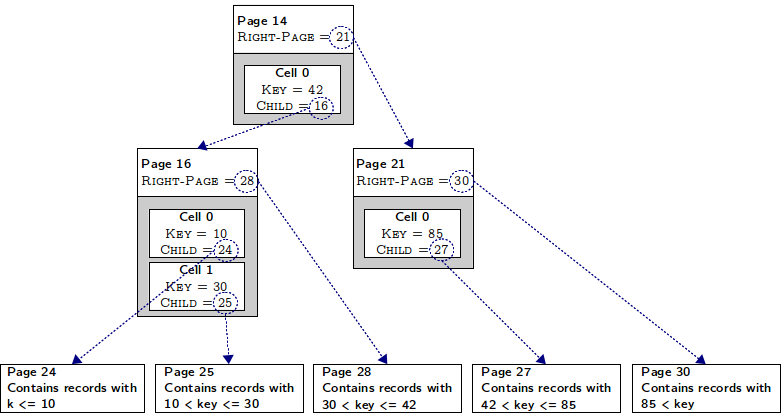
\includegraphics[scale=0.5]{images/sqlite_table_btree.png}
	\caption{Physical layout of table B-Trees \citep{chibd}}
	\label{fig:sqlite_table_btree}
\end{figure}

\subsubsection{Encoding of the data}
\label{subsubsec:sqlite_data_encoding}

Sqlite uses a variable length integer or 'varint' in order encode some of the values inside the database, since they use up less space for small positive values. A varint is a static Huffman encoding of a 64-bit two complements integer. A varint is between and 1 - 9 bytes in size. The maximum number a byte can hold is 127 as the most significant bit is needed as a flag unless we are in the ninth byte where all the bits are used. If the most significant bit is set then we need the next byte. So if it is set in byte 1 then we need byte 2 and so on.
\\\\
If we have the following value in hex 5B and convert this to binary we have 01011011 as we can see the the most significance bit is not set leaving us with the value 91. However, if we have the value in hex 84 and convert this to binary we have the value 10000100, the most significant bit is set this means we need the next byte which has a value in hex of 60 converting this to binary leaves us with  01100000 meaning that this varint is two byes long. In order to create the final value we need to concatenate them together leaving out the most significant bit. creating the value 00001001100000 giving us a total value of 608 in decimal \citep{sausagefactory}. Table~\ref{tbl:varints} show the all combinations of varints. 

\begin{longtable}[h]{| c | c | p{10cm} |}
		\hline
			\textbf{Bytes} & \textbf{Value Range} & \textbf{Bit pattern} \\ 
		\hline
		\endhead
			1 & 7 &  0xxxxxxx \\ \hline
			2 & 14 & 1xxxxxxx 0xxxxxxx\\ \hline
			3 & 21 & 1xxxxxxx 1xxxxxxx 0xxxxxxx\\ \hline
			4 & 28 & 1xxxxxxx 1xxxxxxx 1xxxxxxx 0xxxxxxx\\ \hline
			5 & 35 & 1xxxxxxx 1xxxxxxx 1xxxxxxx 1xxxxxxx 0xxxxxxx\\ \hline
			6 & 42 & 1xxxxxxx 1xxxxxxx 1xxxxxxx 1xxxxxxx 1xxxxxxx 0xxxxxxx\\ \hline
			7 & 49 & 1xxxxxxx 1xxxxxxx 1xxxxxxx 1xxxxxxx 1xxxxxxx 1xxxxxxx 0xxxxxxx\\ \hline
			8 & 56 & 1xxxxxxx 1xxxxxxx 1xxxxxxx 1xxxxxxx 1xxxxxxx 1xxxxxxx 1xxxxxxx 0xxxxxxx\\ \hline
			9 & 64 & 1xxxxxxx 1xxxxxxx 1xxxxxxx 1xxxxxxx 1xxxxxxx 1xxxxxxx 1xxxxxxx 1xxxxxxx xxxxxxxx\\
		\hline
	\caption{Varint combinations \cite{sqliteray}}
	\label{tbl:varints}
\end{longtable}

With this in mind the following pseudo code is needed to decode the varint.

\begin{lstlisting}
	byte[] varints = new byte[9];	// array to store the varints

	for (i = 1 to 9) {	// count the number of bytes
		varints[i] = byte;
		if (bytes most significant is not set) {
			break;
		}
	}
	
	if (number of bytes is 0) {  // check it is a varint.
		return 0;
	} else {
		for (i = 0 to number of bytes) {   // remove significant bit
			varints[i] = varints[i] << 1;
		}
		return concatenation of varints[]; // get the real value
	}
\end{lstlisting}

\subsubsection{B-Tree header}
\label{subsubsec:btree_header}

As mentioned in section~\ref{subsubsec:sqlite_trees_and_cells} the header for each type of B-Tree does not vary that much. Table~\ref{tbl:btree_header} shows the header for the B-Trees.

\begin{longtable}[h]{| c | c | p{10cm} |}
		\hline
			\textbf{Byte Offset} & \textbf{Byte Size} & \textbf{Description} \\ 
		\hline
		\endhead
			0 & 1 & The type of of B-Tree. \newline
			Value of 2 is a interior index B-tree. \newline
			Value of 5 is a interior table B-tree. \newline
			Value of 10 is a Leaf index B-tree. \newline
			Value of 13 is a Leaf table B-tree. \\
		\hline
			1 & 2 & Offset of first freeblock on the page. \\
		\hline
			3 & 2 & Number of cells on page. \\
		\hline
			5 & 2 & Start of content area. A zero is seen as 65536. \\
		\hline
			7 & 1 & Number of fragmented free bytes within the cells. \\
		\hline
			8 & 4 & Interior B-Tree Pages only. The right most pointer. \\ 
		\hline
	\caption{Sqlite B-Tree Header, modified from \cite{sqlite}}
	\label{tbl:btree_header}
\end{longtable}

Immediately following the header is the array of cell pointers, the number of cells is read at offset 3. Each cell pointer is 2 bytes in size. It is worth noting at this point that the pointer and offsets start at the page offset rather then the start of the file, keeping each page self contained. Therefore in order to follow the cell pointers or the other offsets the following sum is needed to calculate its position in the file: 

\begin{lstlisting}	
	cell = ((pageNumer - 1) * pageSize) + offset;
\end{lstlisting}

The right most pointer within interior B-Tree pages is the childs page number not offset therefore to calculate the page offset the following sum is used:

\begin{lstlisting}	
	pageOffset = ((pageNumer - 1) * pageSize);
\end{lstlisting}

\subsubsection{Index B-Tree cell}
\label{subsubsec:index_btree_cell}

As mentioned in section~\ref{subsubsec:sqlite_trees_and_cells} Index B-Tree use the database records as keys. their content also reflects this. Table~\ref{tbl:index_btree_cell} show the layout of the cell:

\begin{longtable}[h]{| c | p{5cm} |}
		\hline
			\textbf{Data type} & \textbf{Description} \\ 
		\hline
		\endhead
			4 byte integer & Page number of child. \newline 
							 Not on leaf cells.\\
		\hline
			Varint & Payload size. \\
		\hline
			byte array & Payload \\
		\hline
			4 byte integer & Page number of overflow \newline
							  Only if payload is to large.\\
		\hline
	\caption{Index B-Tree cell}
	\label{tbl:index_btree_cell}
\end{longtable}

Much like the right child pointer mentioned in section~\ref{subsubsec:btree_header} this is the page number of the child not a pointer. In order to determine if there is a overflow page the following calculation is used:

\begin{lstlisting}	
usable-size = page-size - bytes-of-unused-space;
max-local = (usable-size - 12) * max-embedded-fraction / 255 - 23;

if (payload-size > max-local) {
	we have a overflow page.
}
\end{lstlisting}

Where bytes-of-unused-space is read in the Sqlite header at offset 20 and \newline max-embedded-fraction at offset 12 ( see section~\ref{subsubsec:sqlite_page_hader} for more info ). Once we know there is an offset we can use the following calculation to work out the size of the record in this part of the cell before jumping over to the overflow page:  

\begin{lstlisting}	
usable-size = page-size - bytes-of-unused-space;

min-local = (usable-size - 12) * min-embedded-fraction / 255 - 23;
record-size = min-local + (record-size - min-local) % 
			  (usable-size - 4);

if(record-size > max-local) {
	record-size = min-local;
}
\end{lstlisting}

\subsubsection{Page B-Tree cell}
\label{subsubsec:page_btree_cell}



\subsection{Similar Programs}
\label{subsec:similar_programs}

\subsubsection{Sqlite browser}
\label{subsubsec:sqlite_browser}

One Similar program...
